\documentclass[12pt,aspectratio=169]{beamer}
\usepackage[T1]{fontenc}
\usepackage{lmodern,amsmath,amssymb,booktabs,tikz,graphicx}
\usetikzlibrary{arrows.meta,positioning,calc}
\definecolor{Ink}{HTML}{17324D}
\definecolor{Teal}{HTML}{007F7A}
\definecolor{Muted}{HTML}{556574}
\definecolor{Paper}{HTML}{FAFAF7}
\definecolor{Rust}{HTML}{AD532E}
\definecolor{Gold}{HTML}{B38630}
\setbeamercolor{background canvas}{bg=Paper}
\setbeamercolor{normal text}{fg=Ink}
\setbeamercolor{frametitle}{fg=Ink}
\setbeamercolor{structure}{fg=Teal}
\setbeamercolor{alerted text}{fg=Rust}
\setbeamerfont{frametitle}{size=\LARGE,series=\bfseries}
\setbeamertemplate{navigation symbols}{}
\setbeamersize{text margin left=9mm,text margin right=9mm}
\setbeamertemplate{frametitle}{\par\vspace{2mm}\insertframetitle\par\vspace{1mm}{\color{Gold}\rule{14mm}{1pt}}}
\setbeamertemplate{footline}{\hspace{9mm}\scriptsize\color{Muted}\insertsectionhead\hfill\insertframenumber\hspace{9mm}\vspace{4mm}}
\hypersetup{colorlinks=true,urlcolor=Teal,linkcolor=Muted,pdfauthor={}}
\newcommand{\point}[1]{\par\vspace{3mm}{\large #1\par}}
\newcommand{\eqnote}[1]{\par\vspace{2mm}{\small\color{Muted}#1\par}}
\newcommand{\smalltext}[1]{\eqnote{#1}}
\newcommand{\insight}[1]{\par\vspace{2mm}{\color{Teal}\bfseries #1}\par}
\newcommand{\identity}{\text{\scriptsize accounting identity}}
\newcommand{\policy}{R^{\mathrm{policy}}}
\newcommand{\loanrate}{R^{\mathrm{loan}}}
\newcommand{\nominal}{R^{\mathrm{nom}}}
\newcommand{\realrate}{R^{\mathrm{real}}}
\newcommand{\neutral}{R^{\mathrm{neutral}}}
\newcommand{\spot}[1]{R^{\mathrm{spot}}(#1)}
\newcommand{\forward}[2]{R^{\mathrm{forward}}(#1,#2)}
\newcommand{\bondyield}{R^{\mathrm{bond}}}
\newcommand{\bondrate}[1]{R^{\mathrm{bond}}(#1)}
\AtBeginDocument{\setlength{\abovedisplayskip}{5pt}\setlength{\belowdisplayskip}{5pt}\setlength{\abovedisplayshortskip}{3pt}\setlength{\belowdisplayshortskip}{3pt}}

\hypersetup{pdftitle={Economics and Finance for Mathematicians: Public debt and macro trades}}
\begin{document}

% Slide 1: Public debt and macro trades

\begin{frame}[plain]
{\color{Teal}\large ECONOMICS AND FINANCE\quad /\quad 07}\par\vspace{9mm}{\Huge\bfseries Public debt and macro trades}\par\vspace{7mm}{\Large How do fiscal promises, monetary policy and market prices interact?}
\end{frame}

% Slide 2: Today’s route

\begin{frame}{Today’s route}
\point{Derive the debt ratio before debating debt sustainability.}\point{Distinguish monetary control from fiscal and rollover constraints.}\point{Use dated US/Japan evidence to build conditional trading scenarios.}
\end{frame}

% Slide 3: Debt arithmetic
\section[Debt arithmetic]{Debt arithmetic}
\begin{frame}[plain]
{\color{Gold}\large LECTURE 7}\par\vspace{9mm}{\Huge\bfseries Debt arithmetic}\par\vspace{7mm}{\Large What makes the debt ratio rise or fall?}
\end{frame}

% Slide 4: The government’s one-period financing constraint

\begin{frame}{The government’s one-period financing constraint}
\[B_t=(1+R_t^{\rm debt})B_{t-1}-PB_t.\]\begin{center}\begin{tabular}{@{}ll@{}}\toprule \textbf{Symbol} & \textbf{Meaning}\\\midrule $B_t$ & Nominal debt outstanding after this period\\[2mm]
$R_t^{\rm debt}$ & Effective nominal interest rate on existing debt\\[2mm]
$PB_t$ & Primary surplus: revenues less non-interest spending\\\bottomrule\end{tabular}\end{center}
\end{frame}

% Slide 5: Dividing by nominal GDP

\begin{frame}{Dividing by nominal GDP}
\[d_t\equiv\frac{B_t}{GDP_t^{\rm nominal}},\qquad pb_t\equiv\frac{PB_t}{GDP_t^{\rm nominal}}.\]\[\boxed{d_t=\frac{1+R_t^{\rm debt}}{1+g_t^{\rm nominal}}d_{t-1}-pb_t.}\]\eqnote{$g_t^{\rm nominal}$: nominal GDP growth over the same period.}
\end{frame}

% Slide 6: The interest–growth snowball

\begin{frame}{The interest–growth snowball}
\[\Delta d_t=\frac{R_t^{\rm debt}-g_t^{\rm nominal}}{1+g_t^{\rm nominal}}d_{t-1}-pb_t.\]\point{Interest above growth pushes the ratio up.}\point{A primary surplus pushes the ratio down.}
\end{frame}

% Slide 7: A complete debt-ratio calculation

\begin{frame}{A complete debt-ratio calculation}
\[d_{t-1}=100\%,\quad R^{\rm debt}=6\%,\quad g^{\rm nominal}=3\%,\quad pb=1\%.\]\[\Delta d=\frac{0.06-0.03}{1.03}\times1-0.01=1.91\%\text{ of GDP}.\]\point{The debt ratio rises from 100\% to about 101.91\%.}
\end{frame}

% Slide 8: Growth above interest can permit a primary deficit

\begin{frame}{Growth above interest can permit a primary deficit}
\[R^{\rm debt}=4\%,\quad g^{\rm nominal}=5\%,\quad d_{t-1}=100\%.\]\[pb^{\rm stabilising}=\frac{0.04-0.05}{1.05}\times1=-0.95\%\text{ of GDP}.\]\eqnote{A conditional arithmetic result. Financing risk and future rates remain.}
\end{frame}

% Slide 9: Small parameter differences compound

\begin{frame}{Small parameter differences compound}
\begin{center}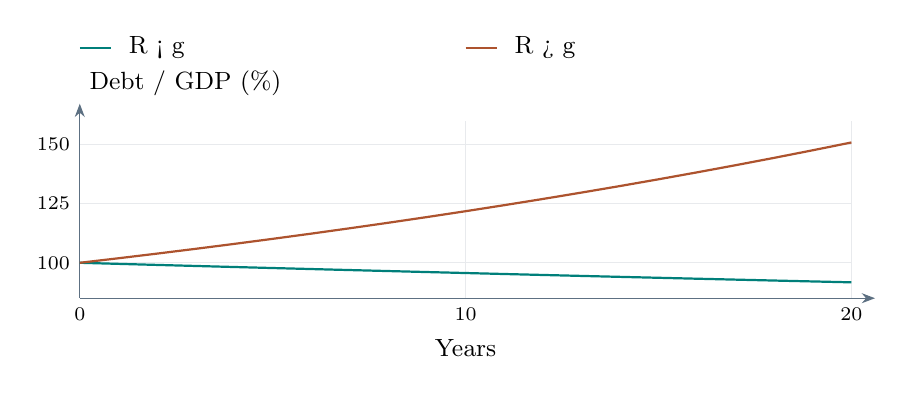
\begin{tikzpicture}[>=Stealth,every node/.style={font=\small}]
\draw[Ink!10] (0.0000,0.0000)--(0.0000,2.2500);\node[below,font=\scriptsize] at (0.0000,0.0000){0};
\draw[Ink!10] (4.9000,0.0000)--(4.9000,2.2500);\node[below,font=\scriptsize] at (4.9000,0.0000){10};
\draw[Ink!10] (9.8000,0.0000)--(9.8000,2.2500);\node[below,font=\scriptsize] at (9.8000,0.0000){20};
\draw[Ink!10] (0.0000,0.4500)--(9.8000,0.4500);\node[left,font=\scriptsize] at (0.0000,0.4500){100};
\draw[Ink!10] (0.0000,1.2000)--(9.8000,1.2000);\node[left,font=\scriptsize] at (0.0000,1.2000){125};
\draw[Ink!10] (0.0000,1.9500)--(9.8000,1.9500);\node[left,font=\scriptsize] at (0.0000,1.9500){150};
\draw[->,Ink!70] (0,0)--(10.100000000000001,0);\draw[->,Ink!70] (0,0)--(0,2.47);
\node[below] at (4.9,-.40){Years};\node[anchor=west] at (0,2.73){Debt / GDP (\%)};
\draw[Teal,thick] plot coordinates {(0.0000,0.4500) (0.4900,0.4364) (0.9800,0.4230) (1.4700,0.4097) (1.9600,0.3965) (2.4500,0.3834) (2.9400,0.3705) (3.4300,0.3577) (3.9200,0.3450) (4.4100,0.3324) (4.9000,0.3200) (5.3900,0.3076) (5.8800,0.2954) (6.3700,0.2833) (6.8600,0.2713) (7.3500,0.2595) (7.8400,0.2477) (8.3300,0.2361) (8.8200,0.2245) (9.3100,0.2131) (9.8000,0.2018)};
\draw[Rust,thick] plot coordinates {(0.0000,0.4500) (0.4900,0.5074) (0.9800,0.5664) (1.4700,0.6272) (1.9600,0.6897) (2.4500,0.7541) (2.9400,0.8203) (3.4300,0.8885) (3.9200,0.9587) (4.4100,1.0308) (4.9000,1.1051) (5.3900,1.1816) (5.8800,1.2603) (6.3700,1.3413) (6.8600,1.4246) (7.3500,1.5104) (7.8400,1.5986) (8.3300,1.6895) (8.8200,1.7829) (9.3100,1.8792) (9.8000,1.9782)};
\draw[Teal,thick] (0.0,3.18)--(0.4,3.18);\node[anchor=west,font=\small] at (0.5,3.18){R < g};
\draw[Rust,thick] (4.9,3.18)--(5.300000000000001,3.18);\node[anchor=west,font=\small] at (5.4,3.18){R > g};
\end{tikzpicture}\end{center}\eqnote{Invented constant paths: green pb = -0.5\%, red pb = +1\% of GDP.}
\end{frame}

% Slide 10: A rising ratio is a warning, not an instant default test

\begin{frame}{A rising ratio is a warning, not an instant default test}
\point{Fiscal adjustment can take time.}\point{Risk depends on the distribution of future funding and primary balances.}\point{Debt definitions and the holder/currency/maturity structure matter.}
\end{frame}

% Slide 11: A long maturity delays the cash-flow effect

\begin{frame}{A long maturity delays the cash-flow effect}
\begin{center}\begin{tabular}{@{}lll@{}}\toprule \textbf{Illustrative refinancing need} & \textbf{Share resetting this year} & \textbf{Rate rise}\\\midrule Mostly short debt & 80\% & +1 point\\[2mm]
Mostly long fixed-rate debt & 10\% & +1 point\\\bottomrule\end{tabular}\end{center}\point{The same market-rate move can have very different near-term budget effects.}
\end{frame}

% Slide 12: Fiscal fatigue and a possible adjustment limit

\begin{frame}{Fiscal fatigue and a possible adjustment limit}
\begin{center}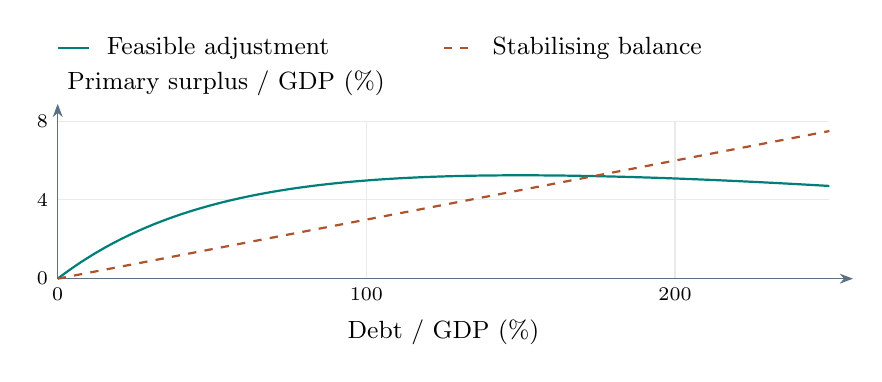
\begin{tikzpicture}[>=Stealth,every node/.style={font=\small}]
\draw[Ink!10] (0.0000,0.0000)--(0.0000,2.0000);\node[below,font=\scriptsize] at (0.0000,0.0000){0};
\draw[Ink!10] (3.9200,0.0000)--(3.9200,2.0000);\node[below,font=\scriptsize] at (3.9200,0.0000){100};
\draw[Ink!10] (7.8400,0.0000)--(7.8400,2.0000);\node[below,font=\scriptsize] at (7.8400,0.0000){200};
\draw[Ink!10] (0.0000,0.0000)--(9.8000,0.0000);\node[left,font=\scriptsize] at (0.0000,0.0000){0};
\draw[Ink!10] (0.0000,1.0000)--(9.8000,1.0000);\node[left,font=\scriptsize] at (0.0000,1.0000){4};
\draw[Ink!10] (0.0000,2.0000)--(9.8000,2.0000);\node[left,font=\scriptsize] at (0.0000,2.0000){8};
\draw[->,Ink!70] (0,0)--(10.100000000000001,0);\draw[->,Ink!70] (0,0)--(0,2.22);
\node[below] at (4.9,-.40){Debt / GDP (\%)};\node[anchor=west] at (0,2.48){Primary surplus / GDP (\%)};
\draw[Teal,thick] plot coordinates {(0.0000,0.0000) (0.0392,0.0297) (0.0784,0.0588) (0.1176,0.0873) (0.1568,0.1152) (0.1960,0.1426) (0.2352,0.1694) (0.2744,0.1957) (0.3136,0.2215) (0.3528,0.2467) (0.3920,0.2714) (0.4312,0.2956) (0.4704,0.3193) (0.5096,0.3426) (0.5488,0.3653) (0.5880,0.3876) (0.6272,0.4095) (0.6664,0.4309) (0.7056,0.4519) (0.7448,0.4724) (0.7840,0.4925) (0.8232,0.5122) (0.8624,0.5315) (0.9016,0.5504) (0.9408,0.5689) (0.9800,0.5871) (1.0192,0.6048) (1.0584,0.6222) (1.0976,0.6393) (1.1368,0.6559) (1.1760,0.6723) (1.2152,0.6883) (1.2544,0.7039) (1.2936,0.7193) (1.3328,0.7343) (1.3720,0.7490) (1.4112,0.7634) (1.4504,0.7775) (1.4896,0.7913) (1.5288,0.8048) (1.5680,0.8180) (1.6072,0.8309) (1.6464,0.8436) (1.6856,0.8560) (1.7248,0.8681) (1.7640,0.8800) (1.8032,0.8916) (1.8424,0.9030) (1.8816,0.9141) (1.9208,0.9250) (1.9600,0.9357) (1.9992,0.9461) (2.0384,0.9563) (2.0776,0.9663) (2.1168,0.9760) (2.1560,0.9856) (2.1952,0.9949) (2.2344,1.0040) (2.2736,1.0130) (2.3128,1.0217) (2.3520,1.0302) (2.3912,1.0385) (2.4304,1.0467) (2.4696,1.0547) (2.5088,1.0625) (2.5480,1.0701) (2.5872,1.0775) (2.6264,1.0848) (2.6656,1.0919) (2.7048,1.0988) (2.7440,1.1056) (2.7832,1.1122) (2.8224,1.1187) (2.8616,1.1250) (2.9008,1.1312) (2.9400,1.1372) (2.9792,1.1431) (3.0184,1.1488) (3.0576,1.1544) (3.0968,1.1598) (3.1360,1.1652) (3.1752,1.1703) (3.2144,1.1754) (3.2536,1.1803) (3.2928,1.1852) (3.3320,1.1898) (3.3712,1.1944) (3.4104,1.1989) (3.4496,1.2032) (3.4888,1.2074) (3.5280,1.2116) (3.5672,1.2156) (3.6064,1.2195) (3.6456,1.2232) (3.6848,1.2269) (3.7240,1.2305) (3.7632,1.2340) (3.8024,1.2374) (3.8416,1.2407) (3.8808,1.2439) (3.9200,1.2470) (3.9592,1.2500) (3.9984,1.2529) (4.0376,1.2558) (4.0768,1.2585) (4.1160,1.2612) (4.1552,1.2638) (4.1944,1.2663) (4.2336,1.2687) (4.2728,1.2710) (4.3120,1.2733) (4.3512,1.2755) (4.3904,1.2776) (4.4296,1.2796) (4.4688,1.2816) (4.5080,1.2835) (4.5472,1.2853) (4.5864,1.2871) (4.6256,1.2887) (4.6648,1.2904) (4.7040,1.2919) (4.7432,1.2934) (4.7824,1.2948) (4.8216,1.2962) (4.8608,1.2975) (4.9000,1.2987) (4.9392,1.2999) (4.9784,1.3011) (5.0176,1.3021) (5.0568,1.3031) (5.0960,1.3041) (5.1352,1.3050) (5.1744,1.3058) (5.2136,1.3066) (5.2528,1.3074) (5.2920,1.3081) (5.3312,1.3087) (5.3704,1.3093) (5.4096,1.3098) (5.4488,1.3103) (5.4880,1.3108) (5.5272,1.3112) (5.5664,1.3115) (5.6056,1.3119) (5.6448,1.3121) (5.6840,1.3123) (5.7232,1.3125) (5.7624,1.3127) (5.8016,1.3128) (5.8408,1.3128) (5.8800,1.3128) (5.9192,1.3128) (5.9584,1.3127) (5.9976,1.3126) (6.0368,1.3125) (6.0760,1.3123) (6.1152,1.3121) (6.1544,1.3118) (6.1936,1.3115) (6.2328,1.3112) (6.2720,1.3109) (6.3112,1.3105) (6.3504,1.3100) (6.3896,1.3096) (6.4288,1.3091) (6.4680,1.3086) (6.5072,1.3080) (6.5464,1.3074) (6.5856,1.3068) (6.6248,1.3061) (6.6640,1.3054) (6.7032,1.3047) (6.7424,1.3040) (6.7816,1.3032) (6.8208,1.3024) (6.8600,1.3016) (6.8992,1.3007) (6.9384,1.2998) (6.9776,1.2989) (7.0168,1.2980) (7.0560,1.2970) (7.0952,1.2960) (7.1344,1.2950) (7.1736,1.2940) (7.2128,1.2929) (7.2520,1.2918) (7.2912,1.2907) (7.3304,1.2895) (7.3696,1.2884) (7.4088,1.2872) (7.4480,1.2859) (7.4872,1.2847) (7.5264,1.2834) (7.5656,1.2822) (7.6048,1.2808) (7.6440,1.2795) (7.6832,1.2782) (7.7224,1.2768) (7.7616,1.2754) (7.8008,1.2740) (7.8400,1.2725) (7.8792,1.2711) (7.9184,1.2696) (7.9576,1.2681) (7.9968,1.2666) (8.0360,1.2650) (8.0752,1.2635) (8.1144,1.2619) (8.1536,1.2603) (8.1928,1.2586) (8.2320,1.2570) (8.2712,1.2553) (8.3104,1.2537) (8.3496,1.2520) (8.3888,1.2503) (8.4280,1.2485) (8.4672,1.2468) (8.5064,1.2450) (8.5456,1.2432) (8.5848,1.2414) (8.6240,1.2396) (8.6632,1.2377) (8.7024,1.2359) (8.7416,1.2340) (8.7808,1.2321) (8.8200,1.2302) (8.8592,1.2283) (8.8984,1.2263) (8.9376,1.2244) (8.9768,1.2224) (9.0160,1.2204) (9.0552,1.2184) (9.0944,1.2164) (9.1336,1.2144) (9.1728,1.2123) (9.2120,1.2102) (9.2512,1.2081) (9.2904,1.2060) (9.3296,1.2039) (9.3688,1.2018) (9.4080,1.1997) (9.4472,1.1975) (9.4864,1.1953) (9.5256,1.1931) (9.5648,1.1909) (9.6040,1.1887) (9.6432,1.1865) (9.6824,1.1842) (9.7216,1.1820) (9.7608,1.1797) (9.8000,1.1774)};
\draw[Rust,dashed,thick] plot coordinates {(0.0000,0.0000) (9.8000,1.8750)};
\draw[Teal,thick] (0.0,2.93)--(0.4,2.93);\node[anchor=west,font=\small] at (0.5,2.93){Feasible adjustment};
\draw[Rust,dashed] (4.9,2.93)--(5.300000000000001,2.93);\node[anchor=west,font=\small] at (5.4,2.93){Stabilising balance};
\end{tikzpicture}\end{center}\eqnote{Invented fiscal-capacity curve and approximate interest–growth gap of 3 points.}
\end{frame}

% Slide 13: Fiscal and monetary interaction
\section[Fiscal and monetary interaction]{Fiscal and monetary interaction}
\begin{frame}[plain]
{\color{Gold}\large LECTURE 7}\par\vspace{9mm}{\Huge\bfseries Fiscal and monetary interaction}\par\vspace{7mm}{\Large Can issuing money remove the government’s real resource constraint?}
\end{frame}

% Slide 14: Nominal repayment and real value are different promises

\begin{frame}{Nominal repayment and real value are different promises}
\point{A government with its own currency can create nominal settlement balances.}\point{It cannot create unlimited real goods by changing nominal units.}\point{Inflation, legal constraints and political choices still affect outcomes.}
\end{frame}

% Slide 15: Fiscal dominance

\begin{frame}{Fiscal dominance}
\point{Debt-financing needs constrain the monetary response to inflation.}\point{A central bank may face pressure to keep financing costs low.}\point{That pressure alone does not prove which policy regime actually prevails.}
\end{frame}

% Slide 16: Inflation can reduce some real debt burdens

\begin{frame}{Inflation can reduce some real debt burdens}
\point{Unexpected inflation erodes the real value of fixed nominal claims.}\point{Indexed debt and new borrowing costs can offset the benefit.}\point{Tax/spending indexation and credibility change the fiscal result.}
\end{frame}

% Slide 17: QE changes the public sector’s liability mix

\begin{frame}{QE changes the public sector’s liability mix}
\begin{center}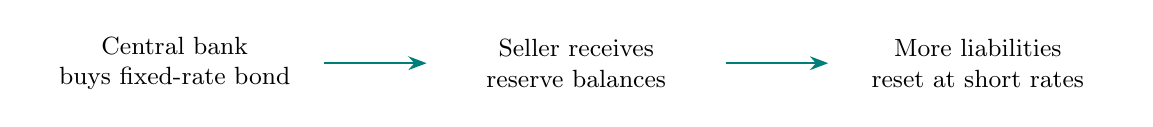
\begin{tikzpicture}[>=Stealth,every node/.style={font=\small,align=center,text width=3.5cm}]\node at (0.0,0){Central bank\\buys fixed-rate bond};\node at (5.1,0){Seller receives\\reserve balances};\node at (10.2,0){More liabilities\\reset at short rates};\draw[->,Teal,thick] (1.9,0)--(3.1999999999999997,0);\draw[->,Teal,thick] (7.0,0)--(8.299999999999999,0);\end{tikzpicture}\end{center}\eqnote{Consolidated exposure depends on reserve remuneration and the full balance sheet.}
\end{frame}

% Slide 18: Fiscal feedback can stabilise debt in a toy model

\begin{frame}{Fiscal feedback can stabilise debt in a toy model}
\[pb_t=a+b\,d_{t-1}.\]\point{$a$: baseline primary balance. $b$: response to inherited debt.}\[d_t=\left[\frac{1+R^{\rm debt}}{1+g^{\rm nominal}}-b\right]d_{t-1}-a.\]
\end{frame}

% Slide 19: Dated US and Japan cases
\section[Dated US and Japan cases]{Dated US and Japan cases}
\begin{frame}[plain]
{\color{Gold}\large LECTURE 7}\par\vspace{9mm}{\Huge\bfseries Dated US and Japan cases}\par\vspace{7mm}{\Large What is verified evidence, and what is a trading hypothesis?}
\end{frame}

% Slide 20: July–August 2026: a common date window

\begin{frame}{July–August 2026: a common date window}
\point{Compare 1 July with 31 August, then inspect the path between them.}\point{Use US Treasury, Japan MOF and ECB daily series.}\point{Keep currencies, yield definitions and local observation times explicit.}
\end{frame}

% Slide 21: Summer 2026: ten-year yield changes

\begin{frame}{Summer 2026: ten-year yield changes}
\begin{center}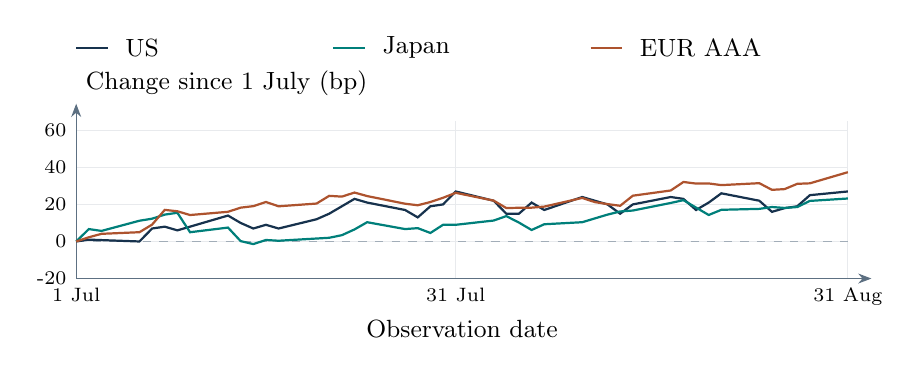
\begin{tikzpicture}[>=Stealth,every node/.style={font=\small}]
\draw[Ink!10] (0.0000,0.0000)--(0.0000,2.0000);\node[below,font=\scriptsize] at (0.0000,0.0000){1 Jul};
\draw[Ink!10] (4.8197,0.0000)--(4.8197,2.0000);\node[below,font=\scriptsize] at (4.8197,0.0000){31 Jul};
\draw[Ink!10] (9.8000,0.0000)--(9.8000,2.0000);\node[below,font=\scriptsize] at (9.8000,0.0000){31 Aug};
\draw[Ink!10] (0.0000,0.0000)--(9.8000,0.0000);\node[left,font=\scriptsize] at (0.0000,0.0000){-20};
\draw[Ink!10] (0.0000,0.4706)--(9.8000,0.4706);\node[left,font=\scriptsize] at (0.0000,0.4706){0};
\draw[Ink!10] (0.0000,0.9412)--(9.8000,0.9412);\node[left,font=\scriptsize] at (0.0000,0.9412){20};
\draw[Ink!10] (0.0000,1.4118)--(9.8000,1.4118);\node[left,font=\scriptsize] at (0.0000,1.4118){40};
\draw[Ink!10] (0.0000,1.8824)--(9.8000,1.8824);\node[left,font=\scriptsize] at (0.0000,1.8824){60};
\draw[->,Ink!70] (0,0)--(10.100000000000001,0);\draw[->,Ink!70] (0,0)--(0,2.22);
\node[below] at (4.9,-.40){Observation date};\node[anchor=west] at (0,2.48){Change since 1 July (bp)};
\draw[Ink!40,dashed] (0.0000,0.4706)--(9.8000,0.4706);
\draw[Ink,thick] plot coordinates {(0.0000,0.4706) (0.1607,0.4941) (0.8033,0.4706) (0.9639,0.6353) (1.1246,0.6588) (1.2852,0.6118) (1.4459,0.6588) (1.9279,0.8000) (2.0885,0.7059) (2.2492,0.6353) (2.4098,0.6824) (2.5705,0.6353) (3.0525,0.7529) (3.2131,0.8235) (3.3738,0.9176) (3.5344,1.0118) (3.6951,0.9647) (4.1770,0.8706) (4.3377,0.7765) (4.4984,0.9176) (4.6590,0.9412) (4.8197,1.1059) (5.3016,0.9882) (5.4623,0.8235) (5.6230,0.8235) (5.7836,0.9647) (5.9443,0.8706) (6.4262,1.0353) (6.5869,0.9882) (6.7475,0.9412) (6.9082,0.8235) (7.0689,0.9412) (7.5508,1.0353) (7.7115,1.0118) (7.8721,0.8706) (8.0328,0.9647) (8.1934,1.0824) (8.6754,0.9882) (8.8361,0.8471) (8.9967,0.8941) (9.1574,0.9176) (9.3180,1.0588) (9.8000,1.1059)};
\draw[Teal,thick] plot coordinates {(0.0000,0.4706) (0.1607,0.6282) (0.3213,0.6047) (0.8033,0.7341) (0.9639,0.7600) (1.1246,0.8118) (1.2852,0.8353) (1.4459,0.5882) (1.9279,0.6471) (2.0885,0.4753) (2.2492,0.4376) (2.4098,0.4894) (2.5705,0.4800) (3.2131,0.5176) (3.3738,0.5506) (3.5344,0.6235) (3.6951,0.7153) (4.1770,0.6282) (4.3377,0.6400) (4.4984,0.5788) (4.6590,0.6824) (4.8197,0.6824) (5.3016,0.7365) (5.4623,0.7929) (5.6230,0.7106) (5.7836,0.6165) (5.9443,0.6894) (6.4262,0.7153) (6.7475,0.8118) (6.9082,0.8518) (7.0689,0.8635) (7.5508,0.9600) (7.7115,0.9953) (7.8721,0.9012) (8.0328,0.8071) (8.1934,0.8729) (8.6754,0.8847) (8.8361,0.9082) (8.9967,0.8965) (9.1574,0.9082) (9.3180,0.9859) (9.8000,1.0165)};
\draw[Rust,thick] plot coordinates {(0.0000,0.4706) (0.1607,0.5241) (0.3213,0.5677) (0.8033,0.5885) (0.9639,0.6847) (1.1246,0.8718) (1.2852,0.8544) (1.4459,0.8066) (1.9279,0.8475) (2.0885,0.9002) (2.2492,0.9193) (2.4098,0.9723) (2.5705,0.9174) (3.0525,0.9523) (3.2131,1.0502) (3.3738,1.0403) (3.5344,1.0919) (3.6951,1.0474) (4.1770,0.9501) (4.3377,0.9306) (4.4984,0.9716) (4.6590,1.0256) (4.8197,1.0885) (5.3016,0.9897) (5.4623,0.8954) (5.6230,0.8985) (5.7836,0.9001) (5.9443,0.9136) (6.4262,1.0236) (6.5869,0.9706) (6.7475,0.9454) (6.9082,0.9239) (7.0689,1.0520) (7.5508,1.1182) (7.7115,1.2263) (7.8721,1.2061) (8.0328,1.2076) (8.1934,1.1865) (8.6754,1.2111) (8.8361,1.1264) (8.9967,1.1357) (9.1574,1.2028) (9.3180,1.2092) (9.8000,1.3506)};
\draw[Ink,thick] (0.0,2.93)--(0.4,2.93);\node[anchor=west,font=\small] at (0.5,2.93){US};
\draw[Teal,thick] (3.266666666666667,2.93)--(3.666666666666667,2.93);\node[anchor=west,font=\small] at (3.766666666666667,2.93){Japan};
\draw[Rust,thick] (6.533333333333334,2.93)--(6.9333333333333345,2.93);\node[anchor=west,font=\small] at (7.033333333333334,2.93){EUR AAA};
\end{tikzpicture}\end{center}\eqnote{Official daily observations, own baseline change. Local closes/fixings differ.}
\end{frame}

% Slide 22: Summer 2026: thirty-year yield changes

\begin{frame}{Summer 2026: thirty-year yield changes}
\begin{center}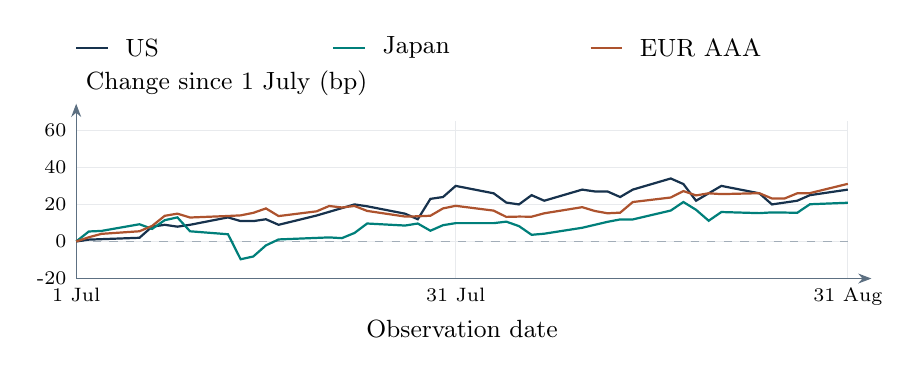
\begin{tikzpicture}[>=Stealth,every node/.style={font=\small}]
\draw[Ink!10] (0.0000,0.0000)--(0.0000,2.0000);\node[below,font=\scriptsize] at (0.0000,0.0000){1 Jul};
\draw[Ink!10] (4.8197,0.0000)--(4.8197,2.0000);\node[below,font=\scriptsize] at (4.8197,0.0000){31 Jul};
\draw[Ink!10] (9.8000,0.0000)--(9.8000,2.0000);\node[below,font=\scriptsize] at (9.8000,0.0000){31 Aug};
\draw[Ink!10] (0.0000,0.0000)--(9.8000,0.0000);\node[left,font=\scriptsize] at (0.0000,0.0000){-20};
\draw[Ink!10] (0.0000,0.4706)--(9.8000,0.4706);\node[left,font=\scriptsize] at (0.0000,0.4706){0};
\draw[Ink!10] (0.0000,0.9412)--(9.8000,0.9412);\node[left,font=\scriptsize] at (0.0000,0.9412){20};
\draw[Ink!10] (0.0000,1.4118)--(9.8000,1.4118);\node[left,font=\scriptsize] at (0.0000,1.4118){40};
\draw[Ink!10] (0.0000,1.8824)--(9.8000,1.8824);\node[left,font=\scriptsize] at (0.0000,1.8824){60};
\draw[->,Ink!70] (0,0)--(10.100000000000001,0);\draw[->,Ink!70] (0,0)--(0,2.22);
\node[below] at (4.9,-.40){Observation date};\node[anchor=west] at (0,2.48){Change since 1 July (bp)};
\draw[Ink!40,dashed] (0.0000,0.4706)--(9.8000,0.4706);
\draw[Ink,thick] plot coordinates {(0.0000,0.4706) (0.1607,0.4941) (0.8033,0.5176) (0.9639,0.6588) (1.1246,0.6824) (1.2852,0.6588) (1.4459,0.6824) (1.9279,0.7765) (2.0885,0.7294) (2.2492,0.7294) (2.4098,0.7529) (2.5705,0.6824) (3.0525,0.8000) (3.2131,0.8471) (3.3738,0.8941) (3.5344,0.9412) (3.6951,0.9176) (4.1770,0.8235) (4.3377,0.7529) (4.4984,1.0118) (4.6590,1.0353) (4.8197,1.1765) (5.3016,1.0824) (5.4623,0.9647) (5.6230,0.9412) (5.7836,1.0588) (5.9443,0.9882) (6.4262,1.1294) (6.5869,1.1059) (6.7475,1.1059) (6.9082,1.0353) (7.0689,1.1294) (7.5508,1.2706) (7.7115,1.2000) (7.8721,0.9882) (8.0328,1.0824) (8.1934,1.1765) (8.6754,1.0824) (8.8361,0.9412) (8.9967,0.9647) (9.1574,0.9882) (9.3180,1.0588) (9.8000,1.1294)};
\draw[Teal,thick] plot coordinates {(0.0000,0.4706) (0.1607,0.5976) (0.3213,0.6047) (0.8033,0.6894) (0.9639,0.6306) (1.1246,0.7412) (1.2852,0.7765) (1.4459,0.6000) (1.9279,0.5624) (2.0885,0.2447) (2.2492,0.2800) (2.4098,0.4212) (2.5705,0.4965) (3.2131,0.5224) (3.3738,0.5129) (3.5344,0.5788) (3.6951,0.6988) (4.1770,0.6729) (4.3377,0.6988) (4.4984,0.6071) (4.6590,0.6776) (4.8197,0.7035) (5.3016,0.7035) (5.4623,0.7224) (5.6230,0.6659) (5.7836,0.5553) (5.9443,0.5694) (6.4262,0.6447) (6.7475,0.7200) (6.9082,0.7506) (7.0689,0.7506) (7.5508,0.8635) (7.7115,0.9718) (7.8721,0.8729) (8.0328,0.7341) (8.1934,0.8447) (8.6754,0.8306) (8.8361,0.8400) (8.9967,0.8376) (9.1574,0.8353) (9.3180,0.9435) (9.8000,0.9624)};
\draw[Rust,thick] plot coordinates {(0.0000,0.4706) (0.1607,0.5245) (0.3213,0.5674) (0.8033,0.6003) (0.9639,0.6683) (1.1246,0.7966) (1.2852,0.8241) (1.4459,0.7750) (1.9279,0.7943) (2.0885,0.8022) (2.2492,0.8342) (2.4098,0.8904) (2.5705,0.7933) (3.0525,0.8533) (3.2131,0.9214) (3.3738,0.9023) (3.5344,0.9215) (3.6951,0.8588) (4.1770,0.7873) (4.3377,0.7903) (4.4984,0.7974) (4.6590,0.8909) (4.8197,0.9235) (5.3016,0.8625) (5.4623,0.7828) (5.6230,0.7867) (5.7836,0.7853) (5.9443,0.8286) (6.4262,0.9063) (6.5869,0.8578) (6.7475,0.8288) (6.9082,0.8365) (7.0689,0.9716) (7.5508,1.0291) (7.7115,1.1110) (7.8721,1.0557) (8.0328,1.0826) (8.1934,1.0722) (8.6754,1.0837) (8.8361,1.0167) (8.9967,1.0166) (9.1574,1.0824) (9.3180,1.0848) (9.8000,1.2027)};
\draw[Ink,thick] (0.0,2.93)--(0.4,2.93);\node[anchor=west,font=\small] at (0.5,2.93){US};
\draw[Teal,thick] (3.266666666666667,2.93)--(3.666666666666667,2.93);\node[anchor=west,font=\small] at (3.766666666666667,2.93){Japan};
\draw[Rust,thick] (6.533333333333334,2.93)--(6.9333333333333345,2.93);\node[anchor=west,font=\small] at (7.033333333333334,2.93){EUR AAA};
\end{tikzpicture}\end{center}\eqnote{Official daily observations, own baseline change. Local closes/fixings differ.}
\end{frame}

% Slide 23: Summer endpoints: yields rose in all three samples

\begin{frame}{Summer endpoints: yields rose in all three samples}
\begin{center}\begin{tabular}{@{}llll@{}}\toprule \textbf{Series} & \textbf{1 July} & \textbf{31 August} & \textbf{Change}\\\midrule US 10-year & 4.480\% & 4.750\% & +27.0 bp\\[2mm]
Japan 10-year & 2.711\% & 2.943\% & +23.2 bp\\[2mm]
EUR AAA 10-year & 2.929\% & 3.303\% & +37.4 bp\\[2mm]
US 30-year & 4.970\% & 5.250\% & +28.0 bp\\[2mm]
Japan 30-year & 3.883\% & 4.092\% & +20.9 bp\\[2mm]
EUR AAA 30-year & 3.379\% & 3.690\% & +31.1 bp\\\bottomrule\end{tabular}\end{center}
\end{frame}

% Slide 24: Summer FX moved on its own path

\begin{frame}{Summer FX moved on its own path}
\begin{center}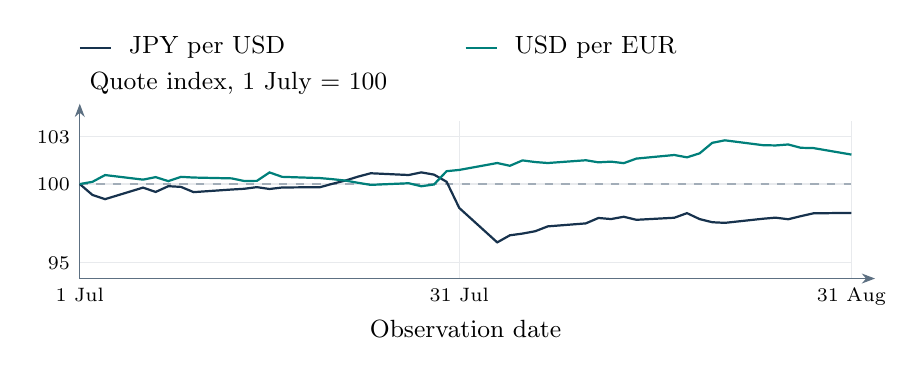
\begin{tikzpicture}[>=Stealth,every node/.style={font=\small}]
\draw[Ink!10] (0.0000,0.0000)--(0.0000,2.0000);\node[below,font=\scriptsize] at (0.0000,0.0000){1 Jul};
\draw[Ink!10] (4.8197,0.0000)--(4.8197,2.0000);\node[below,font=\scriptsize] at (4.8197,0.0000){31 Jul};
\draw[Ink!10] (9.8000,0.0000)--(9.8000,2.0000);\node[below,font=\scriptsize] at (9.8000,0.0000){31 Aug};
\draw[Ink!10] (0.0000,0.2000)--(9.8000,0.2000);\node[left,font=\scriptsize] at (0.0000,0.2000){95};
\draw[Ink!10] (0.0000,1.2000)--(9.8000,1.2000);\node[left,font=\scriptsize] at (0.0000,1.2000){100};
\draw[Ink!10] (0.0000,1.8000)--(9.8000,1.8000);\node[left,font=\scriptsize] at (0.0000,1.8000){103};
\draw[->,Ink!70] (0,0)--(10.100000000000001,0);\draw[->,Ink!70] (0,0)--(0,2.22);
\node[below] at (4.9,-.40){Observation date};\node[anchor=west] at (0,2.48){Quote index, 1 July = 100};
\draw[Ink!40,dashed] (0.0000,1.2000)--(9.8000,1.2000);
\draw[Ink,thick] plot coordinates {(0.0000,1.2000) (0.1607,1.0619) (0.3213,1.0081) (0.8033,1.1547) (0.9639,1.0996) (1.1246,1.1729) (1.2852,1.1639) (1.4459,1.0973) (1.9279,1.1304) (2.0885,1.1399) (2.2492,1.1607) (2.4098,1.1371) (2.5705,1.1563) (3.0525,1.1602) (3.2131,1.2044) (3.3738,1.2445) (3.5344,1.2943) (3.6951,1.3370) (4.1770,1.3147) (4.3377,1.3482) (4.4984,1.3198) (4.6590,1.2286) (4.8197,0.8961) (5.3016,0.4591) (5.4623,0.5491) (5.6230,0.5710) (5.7836,0.6007) (5.9443,0.6626) (6.4262,0.7002) (6.5869,0.7692) (6.7475,0.7554) (6.9082,0.7847) (7.0689,0.7458) (7.5508,0.7720) (7.7115,0.8304) (7.8721,0.7549) (8.0328,0.7150) (8.1934,0.7071) (8.6754,0.7593) (8.8361,0.7732) (8.9967,0.7530) (9.1574,0.7922) (9.3180,0.8283) (9.8000,0.8337)};
\draw[Teal,thick] plot coordinates {(0.0000,1.2000) (0.1607,1.2281) (0.3213,1.3142) (0.8033,1.2562) (0.9639,1.2879) (1.1246,1.2369) (1.2852,1.2914) (1.4459,1.2826) (1.9279,1.2720) (2.0885,1.2387) (2.2492,1.2404) (2.4098,1.3476) (2.5705,1.2914) (3.0525,1.2756) (3.2131,1.2615) (3.3738,1.2439) (3.5344,1.2158) (3.6951,1.1895) (4.1770,1.2105) (4.3377,1.1719) (4.4984,1.1947) (4.6590,1.3634) (4.8197,1.3792) (5.3016,1.4671) (5.4623,1.4319) (5.6230,1.5004) (5.7836,1.4794) (5.9443,1.4671) (6.4262,1.5022) (6.5869,1.4758) (6.7475,1.4846) (6.9082,1.4653) (7.0689,1.5233) (7.5508,1.5690) (7.7115,1.5391) (7.8721,1.5901) (8.0328,1.7236) (8.1934,1.7552) (8.6754,1.6937) (8.8361,1.6902) (8.9967,1.7025) (9.1574,1.6603) (9.3180,1.6568) (9.8000,1.5742)};
\draw[Ink,thick] (0.0,2.93)--(0.4,2.93);\node[anchor=west,font=\small] at (0.5,2.93){JPY per USD};
\draw[Teal,thick] (4.9,2.93)--(5.300000000000001,2.93);\node[anchor=west,font=\small] at (5.4,2.93){USD per EUR};
\end{tikzpicture}\end{center}\eqnote{Different quote directions: lower JPY per USD strengthens yen; higher USD per EUR strengthens euro.}
\end{frame}

% Slide 25: The cross rate checks the currency story

\begin{frame}{The cross rate checks the currency story}
\[\text{JPY per EUR}=(\text{JPY per USD})(\text{USD per EUR}).\]\begin{center}\begin{tabular}{@{}lll@{}}\toprule \textbf{ECB reference observation} & \textbf{1 July} & \textbf{31 August}\\\midrule JPY per USD, derived & 162.71 & 159.73\\[2mm]
USD per EUR & 1.1383 & 1.1596\\[2mm]
JPY per EUR & 185.21 & 185.22\\\bottomrule\end{tabular}\end{center}\eqnote{Endpoint comparison. Small net cross-rate change can hide moves within the window.}
\end{frame}

% Slide 26: A rise in yield is not a flow-of-funds explanation

\begin{frame}{A rise in yield is not a flow-of-funds explanation}
\point{Expected real rates, expected inflation and risk premia can move together.}\point{Hedging costs and relative duration exposure affect investor decisions.}\point{Prices alone do not show which investors repatriated capital.}
\end{frame}

% Slide 27: Exercise: three competing summer explanations

\begin{frame}{Exercise: three competing summer explanations}
\begin{center}\begin{tabular}{@{}p{.46\textwidth}p{.46\textwidth}@{}}\toprule \textbf{Candidate mechanism} & \textbf{What else would you check?}\\\midrule Higher expected future policy rates & Short-rate contracts and policy surprises\\[2mm]
Higher duration / fiscal risk premium & Premium models, supply and risk measures\\[2mm]
Cross-border portfolio adjustment & Hedged returns and actual transaction data\\\bottomrule\end{tabular}\end{center}\eqnote{Several mechanisms may contribute. The daily charts do not choose one automatically.}
\end{frame}

% Slide 28: US policy evidence: September 2026

\begin{frame}{US policy evidence: September 2026}
\point{On 16 September the Fed raised its target range by 0.25 points to 3.75–4.00\%.}\point{The statement described elevated inflation.}\point{The policy decision is one input to pricing the future rate path.}
\end{frame}

% Slide 29: US curve context: 15 October 2026

\begin{frame}{US curve context: 15 October 2026}
\begin{center}\begin{tabular}{@{}ll@{}}\toprule \textbf{Observation} & \textbf{Value}\\\midrule Two-year Treasury par yield & 4.77\%\\[2mm]
Ten-year Treasury par yield & 5.10\%\\[2mm]
Ten minus two-year spread & 33 basis points\\\bottomrule\end{tabular}\end{center}\eqnote{Dated observations. This is a level comparison, not an identified causal decomposition.}
\end{frame}

% Slide 30: Three hypotheses behind a higher US long yield

\begin{frame}{Three hypotheses behind a higher US long yield}
\begin{center}\begin{tabular}{@{}p{.43\textwidth}p{.49\textwidth}@{}}\toprule \textbf{Hypothesis} & \textbf{Evidence to seek}\\\midrule Higher expected policy path & Dated short-rate pricing and announcements\\[2mm]
Higher term/inflation risk premium & Models and inflation-risk indicators\\[2mm]
More duration or funding pressure & Issuance, positioning and market functioning\\\bottomrule\end{tabular}\end{center}\eqnote{Competing explanations, not an attribution of the observed snapshot.}
\end{frame}

% Slide 31: Japan policy evidence: September 2026

\begin{frame}{Japan policy evidence: September 2026}
\point{The 18 September BoJ decision set the overnight call-rate guideline at around 1.25\%.}\point{The new guideline took effect on 24 September.}\point{A higher short rate is one component of normalisation.}
\end{frame}

% Slide 32: Japan: the JGB purchase plan

\begin{frame}{Japan: the JGB purchase plan}
\begin{center}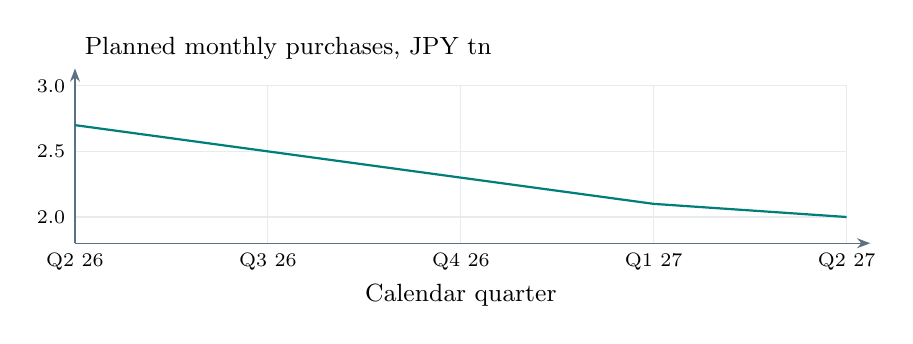
\begin{tikzpicture}[>=Stealth,every node/.style={font=\small}]
\draw[Ink!10] (0.0000,0.0000)--(0.0000,2.0000);\node[below,font=\scriptsize] at (0.0000,0.0000){Q2 26};
\draw[Ink!10] (2.4500,0.0000)--(2.4500,2.0000);\node[below,font=\scriptsize] at (2.4500,0.0000){Q3 26};
\draw[Ink!10] (4.9000,0.0000)--(4.9000,2.0000);\node[below,font=\scriptsize] at (4.9000,0.0000){Q4 26};
\draw[Ink!10] (7.3500,0.0000)--(7.3500,2.0000);\node[below,font=\scriptsize] at (7.3500,0.0000){Q1 27};
\draw[Ink!10] (9.8000,0.0000)--(9.8000,2.0000);\node[below,font=\scriptsize] at (9.8000,0.0000){Q2 27};
\draw[Ink!10] (0.0000,0.3333)--(9.8000,0.3333);\node[left,font=\scriptsize] at (0.0000,0.3333){2.0};
\draw[Ink!10] (0.0000,1.1667)--(9.8000,1.1667);\node[left,font=\scriptsize] at (0.0000,1.1667){2.5};
\draw[Ink!10] (0.0000,2.0000)--(9.8000,2.0000);\node[left,font=\scriptsize] at (0.0000,2.0000){3.0};
\draw[->,Ink!70] (0,0)--(10.100000000000001,0);\draw[->,Ink!70] (0,0)--(0,2.22);
\node[below] at (4.9,-.40){Calendar quarter};\node[anchor=west] at (0,2.48){Planned monthly purchases, JPY tn};
\draw[Teal,thick] plot coordinates {(0.0000,1.5000) (2.4500,1.1667) (4.9000,0.8333) (7.3500,0.5000) (9.8000,0.3333)};
\end{tikzpicture}\end{center}\eqnote{BoJ plan announced 16 June 2026. Planned amounts, not realised purchases.}
\end{frame}

% Slide 33: Why Japanese capital need not immediately return home

\begin{frame}{Why Japanese capital need not immediately return home}
\point{Domestic yields, hedging costs and expected FX returns all matter.}\point{Hedged foreign bonds retain interest-rate and spread exposure.}\point{Mandates, liabilities and existing hedges affect portfolio changes.}
\end{frame}

% Slide 34: A hedge-cost illustration

\begin{frame}{A hedge-cost illustration}
\[R^{\rm JPY}=1\%,\quad R^{\rm USD}=4\%,\quad E=150\;\text{JPY per USD}.\]\[F=150\frac{1.01}{1.04}=145.67\;\text{JPY per USD}.\]\point{A covered one-year USD deposit returns 1\% in yen under parity.}
\end{frame}

% Slide 35: US/Japan counterfactuals

\begin{frame}{US/Japan counterfactuals}
\begin{center}\begin{tabular}{@{}p{.43\textwidth}p{.49\textwidth}@{}}\toprule \textbf{Shock relative to expectations} & \textbf{Conditional channel}\\\midrule BoJ path reprices higher & JPY carry funding becomes less attractive\\[2mm]
JGB term premium rises & Long JGB prices fall at fixed cash flows\\[2mm]
Global risk appetite collapses & Positions may unwind and premia change\\\bottomrule\end{tabular}\end{center}\eqnote{Scenarios for reasoning, not predictions or descriptions of a realised event.}
\end{frame}

% Slide 36: A macro trading lab
\section[A macro trading lab]{A macro trading lab}
\begin{frame}[plain]
{\color{Gold}\large LECTURE 7}\par\vspace{9mm}{\Huge\bfseries A macro trading lab}\par\vspace{7mm}{\Large How does a conditional view become a sized position?}
\end{frame}

% Slide 37: Markets react to the surprise in the full announcement

\begin{frame}{Markets react to the surprise in the full announcement}
\point{A 0.25-point cut was expected. A 0.50-point cut arrives.}\point{The decision is 0.25 points more dovish than expected.}\point{Guidance and economic news can change the later path too.}
\end{frame}

% Slide 38: Exercise: a cut today, but a higher long yield?

\begin{frame}{Exercise: a cut today, but a higher long yield?}
\point{After the announcement, assume:}\point{Expected average short rate over ten years rises 0.10 points.}\point{The ten-year term premium rises 0.20 points.}\eqnote{What happens to the ten-year yield? What about a duration-8 bond?}
\end{frame}

% Slide 39: The decomposition gives the answer

\begin{frame}{The decomposition gives the answer}
\[\Delta\spot{10}\approx0.10+0.20=0.30\text{ percentage points}.\]\[\frac{\Delta P}{P}\approx-8\times0.003=-2.4\%.\]\point{The long yield rises and the bond loses value\par in this specified scenario.}
\end{frame}

% Slide 40: Turn a headline into a conditional chain

\begin{frame}{Turn a headline into a conditional chain}
\point{Identify the shock and the prior expectation.}\point{State the model and policy response.}\point{Translate the view into dated cash flows and yield changes.}\point{Size the exposure and test the counterfactual.}
\end{frame}

% Slide 41: Final exercise: a trade needs a falsifiable claim

\begin{frame}{Final exercise: a trade needs a falsifiable claim}
\point{Choose a shock, prior pricing and a policy response.}\point{Predict two yields and one exchange rate, with assumptions.}\point{Size the trade and name the counterfactual that would make it lose.}
\end{frame}

% Slide 42: Further reading
\section[Reading]{Reading}
\begin{frame}{Further reading}
\point{Dmitriy Sergeyev, Bocconi 30054 course materials.}\point{Krugman, Obstfeld \& Melitz, \emph{International Economics}.}\point{Source links and worked answers accompany each slide in the notes.}
\end{frame}
\end{document}
